% Options for packages loaded elsewhere
\PassOptionsToPackage{unicode}{hyperref}
\PassOptionsToPackage{hyphens}{url}
\PassOptionsToPackage{dvipsnames,svgnames,x11names}{xcolor}
\documentclass[
  11pt,
]{article}
\usepackage{xcolor}
\usepackage[margin=0.85in]{geometry}
\usepackage{amsmath,amssymb}
\setcounter{secnumdepth}{-\maxdimen} % remove section numbering
\usepackage{iftex}
\ifPDFTeX
  \usepackage[T1]{fontenc}
  \usepackage[utf8]{inputenc}
  \usepackage{textcomp} % provide euro and other symbols
\else % if luatex or xetex
  \usepackage{unicode-math} % this also loads fontspec
  \defaultfontfeatures{Scale=MatchLowercase}
  \defaultfontfeatures[\rmfamily]{Ligatures=TeX,Scale=1}
\fi
\usepackage{lmodern}
\ifPDFTeX\else
  % xetex/luatex font selection
\fi
% Use upquote if available, for straight quotes in verbatim environments
\IfFileExists{upquote.sty}{\usepackage{upquote}}{}
\IfFileExists{microtype.sty}{% use microtype if available
  \usepackage[]{microtype}
  \UseMicrotypeSet[protrusion]{basicmath} % disable protrusion for tt fonts
}{}
\makeatletter
\@ifundefined{KOMAClassName}{% if non-KOMA class
  \IfFileExists{parskip.sty}{%
    \usepackage{parskip}
  }{% else
    \setlength{\parindent}{0pt}
    \setlength{\parskip}{6pt plus 2pt minus 1pt}}
}{% if KOMA class
  \KOMAoptions{parskip=half}}
\makeatother
\usepackage{longtable,booktabs,array}
\newcounter{none} % for unnumbered tables
\usepackage{calc} % for calculating minipage widths
% Correct order of tables after \paragraph or \subparagraph
\usepackage{etoolbox}
\makeatletter
\patchcmd\longtable{\par}{\if@noskipsec\mbox{}\fi\par}{}{}
\makeatother
% Allow footnotes in longtable head/foot
\IfFileExists{footnotehyper.sty}{\usepackage{footnotehyper}}{\usepackage{footnote}}
\makesavenoteenv{longtable}
\usepackage{graphicx}
\makeatletter
\newsavebox\pandoc@box
\newcommand*\pandocbounded[1]{% scales image to fit in text height/width
  \sbox\pandoc@box{#1}%
  \Gscale@div\@tempa{\textheight}{\dimexpr\ht\pandoc@box+\dp\pandoc@box\relax}%
  \Gscale@div\@tempb{\linewidth}{\wd\pandoc@box}%
  \ifdim\@tempb\p@<\@tempa\p@\let\@tempa\@tempb\fi% select the smaller of both
  \ifdim\@tempa\p@<\p@\scalebox{\@tempa}{\usebox\pandoc@box}%
  \else\usebox{\pandoc@box}%
  \fi%
}
% Set default figure placement to htbp
\def\fps@figure{htbp}
\makeatother
\setlength{\emergencystretch}{3em} % prevent overfull lines
\providecommand{\tightlist}{%
  \setlength{\itemsep}{0pt}\setlength{\parskip}{0pt}}
% Make wide tables fit: small font inside longtables/tabulars, allow wrapping.
\usepackage{etoolbox}
\AtBeginEnvironment{longtable}{\footnotesize}
\AtBeginEnvironment{tabular}{\footnotesize}
\usepackage{bookmark}
\IfFileExists{xurl.sty}{\usepackage{xurl}}{} % add URL line breaks if available
\urlstyle{same}
\hypersetup{
  colorlinks=true,
  linkcolor={blue},
  filecolor={Maroon},
  citecolor={Blue},
  urlcolor={blue},
  pdfcreator={LaTeX via pandoc}}

\author{}
\date{}

\begin{document}

\section{The Perceptibility Gap and the Expandable
Human Codec: A Two-Study Preregistered Program for
Measuring Human-Compatible Reach
Frontiers}\label{the-perceptibility-gap-and-the-expandable-human-codec-a-two-study-preregistered-program-for-measuring-human-compatible-reach-frontiers}

Wayne A. Satz, MD\\
Director of Clinical Informatics, Department of
Emergency Medicine, Temple University Health System\\
ORCID: 0000-0003-3090-3852\\
Manuscript v1.4. Preregistered program. May 30, 2026.\\
Extends: \emph{The Codec Ceiling} (Satz, 2026).
Supersedes v1.3; changes summarized in Section 0.

\subsection{Abstract}\label{abstract}

Quantitative accounts often define superintelligence as
superior problem-solving across domains. This
manuscript proposes a complementary structural account:
a system becomes superintelligence-relevant for human
oversight when it forms machine-native distinctions
that cannot be faithfully compressed into unaided human
channels. At that point ordinary explanation risks
becoming a lossy projection rather than genuine
perception, producing \emph{false transparency} -
fluent summaries mistaken for understanding.

The work does not attempt to prove that broad thesis.
It tests the minimal empirical bridge the thesis
requires. Study 1 establishes a rate-distortion
frontier for machine representations of held-out
dynamical trajectories while separating two variables
that are often conflated: channel throughput and the
repertoire of distinctions a codec resolves. The source
family is now hierarchical: a linear coupled-oscillator
family remains the calibration and ablation medium,
while a simulated magnetic-pendulum family is added as
the nonlinear stress test for the two places the linear
medium is weakest - non-native latent access and
dimensionality scaling. Study 2 reuses the same
held-out source families and converts all outcomes to a
common relative-distortion scale, asking whether a
trained human using an artificial tactile channel
carrying a simulator-known latent variable can move
measurably along the same frontier.

The primary addition target is not raw bitrate. It is
acquisition of task-relevant distinctions: a
basin-of-attraction latent,
boundary-proximity/divergence information, and their
downstream use in prediction under native-vision
limits. A developmental proof-ladder validates the
runnable design in silico before human recruitment;
those numbers are treated as a smoke test, not
inferential evidence. Success would not show that
humans can understand arbitrary superintelligence. It
would show the narrower, tractable result: human
representational reach can be experimentally expanded
and measured under controlled conditions. The safety
implication is also narrow: single-channel explanations
should be supplemented by measurable multi-codec audit
signals, not replaced by a presumed solution to
alignment.

\textbf{Keywords:} superintelligence; codec ceiling;
sensory addition; rate-distortion; chaotic dynamics;
basin of attraction; AI safety; perceptibility;
vibrotactile learning; preregistration

\begin{center}\rule{0.5\linewidth}{0.5pt}\end{center}

\subsection{0. Changes across v1.2, v1.3, and v1.4, and
why}\label{changes-across-v1.2-v1.3-and-v1.4-and-why}

\subsubsection{0.0 What v1.4 changes (cross-family
generalization)}\label{what-v1.4-changes-cross-family-generalization}

v1.4 closes the single largest remaining limitation of
the developmental skeleton noted in v1.3 Appendix F.5:
every developmental gate ran on \textbf{one} source
family at a time, so a PASS could not demonstrate
cross-family reach. The developmental code now runs the
full ladder and codec contest across a registry of
source families behind a single configuration switch,
and reports a \textbf{gate matrix} marking which gates
are family-robust (PASS on at least two families)
versus family-specific. A second continuous family was
added - a Duffing-type \textbf{nonlinear oscillator}
(cubic stiffness) sharing the linear family's
observable shape - alongside the existing linear
calibration family. A regression fixture freezes the
linear numbers so the refactor cannot silently change
them, and a per-family no-leakage test makes the v1.3
leakage class (F.1) un-reintroducible as families are
added.

Result on eight seeds: \textbf{seven of nine gates
(S0-S4, S6, S8) are family-robust}. Two findings are
new and reported honestly: \textbf{S5 (additive access)
is family-specific} - it carries no unique signal on
the linear family but PASSES on the nonlinear family,
where cubic interaction makes cross-oscillator coupling
genuinely informative; and \textbf{S7 (dimensionality
slope) fails on both families}, because
engineered-feature count grows with oscillator count
faster than the nonlinearity adds difficulty. No gate
threshold was tuned per family. Details in Section 5.1
and Appendix F.6.

\subsubsection{0.1 What v1.3 changes (integrity
revision)}\label{what-v1.3-changes-integrity-revision}

v1.3 is an integrity revision triggered by an
adversarial re-audit of the developmental code, not a
change to the confirmatory design or claim ladder.
After the audit, the developmental bundle was re-run on
eight seeds with corrected controls. Six changes
follow.

\begin{enumerate}
\def\labelenumi{\arabic{enumi}.}
\tightlist
\item
  \textbf{Developmental ``additive-access'' leakage
  removed.} The earlier developmental magnetic-pendulum
  ``expanded'' channel concatenated a noisy copy of the
  prediction target (basin label and finite-time
  divergence) into its own input features. This was
  label leakage: a channel built only from the leaked
  target reached the noise ceiling
  \texttt{1\ -\ flip\_prob} with zero physics. The
  leaked channel is retained \textbf{only} as an
  explicitly labeled
  \texttt{oracle\_leak\_positive\_control}; the honest
  developmental comparison now uses an
  \texttt{expanded\_physics} channel built solely from
  additional real preview observables (velocity
  profile, radial dynamics, cross-coordinate
  interaction moments) that contain no target. This
  corrects a developmental result, not a confirmatory
  one, but the confirmatory tactile mapping (Appendix
  A) inherits the same discipline: an encoded latent
  may never be the answer label itself.
\item
  \textbf{Additive-access control hardened.} The
  developmental additive-access proxy (S5) previously
  used an independent train/test reshuffle as its sham.
  v1.3 replaces it with a distribution-preserving
  phase-randomized surrogate and adds a
  unique-contribution test (does the candidate channel
  predict the residual left by the native channel). On
  the linear family this test now returns no unique
  signal, which is reported as an honest negative.
\item
  \textbf{Multi-codec audit de-tautologized.} The
  developmental audit correlation is now accompanied by
  a leave-one-codec-out (LOCO) estimate, in which a
  held-out codec's error is predicted from the
  disagreement of the \emph{other} codecs only, plus a
  permutation null. Both confirm the developmental
  disagreement-error signal is not a
  std/\textbar mean-truth\textbar{} artifact.
\item
  \textbf{Per-target and across-seed reporting.}
  Developmental recovery is now reported per target (so
  a strong mean cannot hide an unlearned parameter) and
  with across-seed standard deviations; developmental
  seeds raised from two to eight.
\item
  \textbf{Estimators stated as run.} The developmental
  proof-ladder runs scikit-learn Ridge (continuous
  targets) and a distance-weighted k-nearest-neighbor
  classifier/regressor (categorical basin and
  divergence). The MLP and small-Transformer estimators
  named in the confirmatory methods are \textbf{planned
  confirmatory analyses that have not yet been run};
  the manuscript labels them as such and does not
  report numbers from them.
\item
  \textbf{Reproducibility fixes.} The shared-axis
  figure reference is corrected to the deposited
  filename, and an integrity-audit appendix (Appendix
  F) records the findings, the mitigations, and the
  re-run evidence.
\end{enumerate}

The v1.3 developmental numbers in Section 5 and
Appendix F supersede the v1.2b table. No Tier 1-3
claim, hypothesis, power target, or equivalence margin
changed.

\subsubsection{0.2 What v1.2 changed
(retained)}\label{what-v1.2-changed-retained}

v1.1a made the right substantive move by adding a
nonlinear magnetic-pendulum source family, an
executable proof-ladder, and concrete HE2/HE5
operationalizations. v1.2 kept those gains but added
seven safeguards that make the manuscript harder to
overread.

\begin{enumerate}
\def\labelenumi{\arabic{enumi}.}
\tightlist
\item
  \textbf{Source-family hierarchy, not uncontrolled
  expansion.} The linear oscillator is the calibration
  and ablation medium. The magnetic pendulum is the
  confirmatory nonlinear stress test for HE2 and HE4,
  not a license to broaden every claim.
\item
  \textbf{Normalized distortion replaces an ambiguous
  single-axis claim.} Continuous outcomes use nRMSE,
  categorical basin outcomes use log-loss or Brier
  score, and all are plotted as relative distortion,
  \texttt{D\ =\ loss(channel)\ /\ loss(uninformative)},
  with \texttt{rho\ =\ 1\ -\ D}. This preserves the
  shared axis without pretending that nRMSE and
  log-loss are the same quantity.
\item
  \textbf{Native-invisibility is validated, not
  assumed.} A latent counts as non-native only if
  preregistered unaided-vision baselines fail to
  recover it reliably at the displayed preview
  duration. Otherwise it is demoted to a substitution
  or assistive-information condition.
\item
  \textbf{Complexity is measured, not assumed from
  magnet count.} Candidate \texttt{m\ =\ 3,\ 4,\ 5}
  magnetic-pendulum configurations are accepted for HE4
  only if calibrated basin entropy, boundary density,
  uncertainty exponent, or finite-time divergence
  statistics produce an ordered difficulty gradient.
\item
  \textbf{The proof-ladder is demoted to developmental
  evidence.} The pass pattern (seven of nine after the
  v1.3 corrections; see Section 5) is useful because it
  documents implementation behavior and exposes the
  informative S5 and S7 failures. It is not reported as
  confirmatory evidence.
\item
  \textbf{HE2 is split into decoding and use.}
  Participants must decode the added latent and show
  downstream predictive benefit on held-out or
  near-boundary trials. This prevents direct label
  transmission from being mistaken for full
  representational acquisition.
\item
  \textbf{Power and TOST language are made internally
  consistent.} The target is 90-105 completers,
  implying higher enrollment under 25-30\% attrition.
  Equivalence margins are frozen before confirmatory
  analysis and reported with sensitivity checks.
\end{enumerate}

The claim ladder, scope discipline, and refusal of
survival/silver-bullet claims remain unchanged.

\begin{center}\rule{0.5\linewidth}{0.5pt}\end{center}

\subsection{0b. Contributions: what the experiments are
designed to
add}\label{b.-contributions-what-the-experiments-are-designed-to-add}

The following are proposed contributions conditional on
successful completion of the preregistered studies, not
claims already established by the protocol.

\begin{itemize}
\tightlist
\item
  \textbf{Unification.} The program is designed to
  place a trained human perceptual channel on the same
  normalized rate-distortion axis used to evaluate
  machine-native channels (HE3).
\item
  \textbf{Addition, not mere substitution.} The human
  study tests whether participants can acquire and use
  a simulator-known latent that is not reliably
  recoverable from the native display under the
  preregistered preview conditions (HE2).
\item
  \textbf{The lever tested with ground truth.} Study 1
  separates distinctions from throughput by varying
  quantization structure and channel budget
  independently (S1-H1/H2/H3).
\item
  \textbf{A scaling slope for human codec expansion.}
  The nonlinear stress test estimates whether acquired
  distinctions degrade as measured dynamical complexity
  rises (HE4).
\item
  \textbf{A measurable audit primitive.} HE5 converts
  the safety intuition of false transparency into
  measurable signals: disagreement-error correlation,
  top-error detection AUC, and reduction in undetected
  high-error cases.
\item
  \textbf{A reusable benchmark scaffold.} The
  simulator, proof-ladder, and tactile-channel protocol
  are specified so other labs can replicate, falsify,
  or extend the program on consumer hardware.
\end{itemize}

\begin{center}\rule{0.5\linewidth}{0.5pt}\end{center}

\subsection{Scope of the claim: reach frontiers, not
survival
theorems}\label{scope-of-the-claim-reach-frontiers-not-survival-theorems}

The work does \textbf{not} claim that biological
integration is necessary for human survival, that any
single interface program is a privileged route to
alignment, or that codec contrast is a complete safety
solution. Those claims exceed the evidential scope of
the studies.

The claim is narrower. Human-compatible representations
have measurable \textbf{reach frontiers}: regions of
structure recoverable, learnable, or auditable through
a given codec. Sensory substitution and
artificial-channel training show that these frontiers
can move, but not that they can move arbitrarily,
quickly, or far enough for every future system. The
experiments test a bounded question: whether trained
artificial channels expand the set of distinctions
humans recover from controlled dynamical systems,
measured on a shared relative-distortion axis.

The binding limitation is a \textbf{distinction limit},
not merely a scalar bitrate limit. A representation
becomes human-inaccessible when its operative contrasts
cannot be learned, stabilized, or used, even if a
compressed signal can still be transmitted. Throughput
matters for real-time exchange; the prior question is
whether the receiver has the distinctions at all.

\textbf{Three claims are explicitly excluded} from the
confirmatory program: (1) \emph{immediate invisibility}
- we claim a sufficiently advanced system may become
operationally non-auditable through ordinary channels,
not invisible the moment it exists; (2)
\emph{single-program necessity} - bidirectional BCI is
one route within a broader portfolio; (3) \emph{fixed
human constants} - the approximately 39 bits/s and
approximately 10 bits/s figures are empirical
estimates, and the argument depends only on the
qualitative human-machine gap.

\subsubsection{Claim ladder}\label{claim-ladder}

{\def\LTcaptype{none} % do not increment counter
\begin{longtable}[]{@{}
  >{\raggedright\arraybackslash}p{(\linewidth - 4\tabcolsep) * \real{0.3333}}
  >{\raggedright\arraybackslash}p{(\linewidth - 4\tabcolsep) * \real{0.3333}}
  >{\raggedright\arraybackslash}p{(\linewidth - 4\tabcolsep) * \real{0.3333}}@{}}
\toprule\noalign{}
\begin{minipage}[b]{\linewidth}\raggedright
Tier
\end{minipage} &
\begin{minipage}[b]{\linewidth}\raggedright
License
\end{minipage} &
\begin{minipage}[b]{\linewidth}\raggedright
Examples
\end{minipage} \\
\midrule\noalign{}
\endhead
\bottomrule\noalign{}
\endlastfoot
Tier 1 & Directly tested in the benchmark &
Distinctions predict recovery better than raw I/O after
intake saturation; trained participants acquire and use
a non-native latent under controlled conditions. \\
Tier 2 & Cross-study inference from aligned metrics &
The trained-human channel can be placed on the machine
relative-distortion axis; repertoire can expand while
central integration rate remains limiting. \\
Tier 3 & Structural / safety extrapolation &
Superintelligence may outgrow unaided human audit;
multi-codec contrast is a candidate audit layer, not a
solution. \\
\end{longtable}
}

Stronger claims cannot be rescued by weaker evidence:
later hypotheses are gated by earlier ones, and Tier 3
claims remain conditional.

\begin{center}\rule{0.5\linewidth}{0.5pt}\end{center}

\subsection{1. The codec ceiling and the two human
ceilings}\label{the-codec-ceiling-and-the-two-human-ceilings}

An observer renders a world through a codec
\texttt{C\ =\ \{S,\ M,\ R,\ P,\ A\}}: sensing,
measurement basis, record, predictive model, and
action. The ceiling it meets is set by the distinctions
the codec makes available, not by the bits a channel
can push.

The human codec has two relevant ceilings. The
\textbf{peripheral codec} - the repertoire of
distinctions - is the set of contrasts an observer can
resolve, learn, and stabilize. It is expandable through
training, tools, and sensory substitution; it is a
movable reach frontier. The \textbf{central codec} -
the integration rate - is the rate at which resolved
distinctions are bound into conscious,
decision-relevant structure. High-level behavior
occupies a low-rate regime relative to raw intake
(Zheng \& Meister, 2025), is harder to move, and
becomes the next constraint after the repertoire is
enlarged.

Perceptibility \texttt{rho} is therefore primarily a
repertoire question. Expanding a codec can add
distinctions and raise \texttt{rho} without raising
central speed. The central ceiling then limits
real-time depth, not whether structure is perceivable
in principle. This is why throughput-centric responses
to opacity - more tokens, bigger context, richer
dashboards - can fail: a wider pipe does not decode an
unknown codebook.

\begin{center}\rule{0.5\linewidth}{0.5pt}\end{center}

\subsection{2. The Human Codec Expansion Proposition
(Tier 3 structural
argument)}\label{the-human-codec-expansion-proposition-tier-3-structural-argument}

A superintelligent system may form internal
distinctions not natively represented in human
channels. If its relevant state-space grows faster than
the human channel can decode, oversight collapses into
summaries - useful, but not perception of operative
structure. Preserving human agency then requires at
least one of three strategies: (1) slow the system to
human-auditable speed, sacrificing speed; (2) restrict
it to human-native representations, sacrificing
machine-native intelligence; or (3) expand the human
codec, attempting to preserve both capability and
agency. This is argued, not demonstrated.

The empirical question is narrower: \textbf{can
training plus an artificial channel move humans along
the same rate-distortion frontier used to measure
machine-native representations?} Study 2 is designed to
answer that question, not the full superintelligence
thesis.

\begin{center}\rule{0.5\linewidth}{0.5pt}\end{center}

\subsection{3. Cosmological intuition as exposition,
not evidence - and the Lyapunov
caveat}\label{cosmological-intuition-as-exposition-not-evidence---and-the-lyapunov-caveat}

Cosmological metaphors - expanding space, event
horizons, the ``cosmic straw'' - are intuition pumps,
not evidence. The benchmark lives entirely in
\textbf{reach-frontier space}: ground truth is always
available, so it does not instantiate a causal horizon.
\texttt{direct\_archmatch} is an empirical
\textbf{information ceiling} for the supplied data, not
a speed-of-light or event-horizon analog.

{\def\LTcaptype{none} % do not increment counter
\begin{longtable}[]{@{}
  >{\raggedright\arraybackslash}p{(\linewidth - 4\tabcolsep) * \real{0.3333}}
  >{\raggedright\arraybackslash}p{(\linewidth - 4\tabcolsep) * \real{0.3333}}
  >{\raggedright\arraybackslash}p{(\linewidth - 4\tabcolsep) * \real{0.3333}}@{}}
\toprule\noalign{}
\begin{minipage}[b]{\linewidth}\raggedright
Cosmological intuition
\end{minipage} &
\begin{minipage}[b]{\linewidth}\raggedright
Benchmark object
\end{minipage} &
\begin{minipage}[b]{\linewidth}\raggedright
Correct reading
\end{minipage} \\
\midrule\noalign{}
\endhead
\bottomrule\noalign{}
\endlastfoot
Reach frontier (movable) & The entire benchmark axis &
What every tested channel occupies. \\
Information ceiling (\texttt{direct\_archmatch}) & Best
recoverable from the supplied data & Reach-frontier
best case, not the speed of light. \\
Worse channel (symbolic) & Human-readable compression &
A worse, movable reach frontier, not a horizon. \\
Event horizon / speed of light & No benchmark analog &
Ground truth is always available by design. \\
\end{longtable}
}

\textbf{Chaos discipline.} In a chaotic system,
prediction error grows exponentially past the Lyapunov
time for every codec, including the machine. A task
that floors all codecs discriminates nothing. The
nonlinear benchmark therefore targets only well-posed
quantities: generative parameters, basin label,
boundary proximity, finite-time divergence, and
short-horizon prediction within the preregistered
Lyapunov window. It never treats long-horizon
exact-path reconstruction as a primary endpoint.

\textbf{Physical pendulum discipline.} A physical
magnetic pendulum may be useful for demonstration and
recruitment materials, but not for confirmatory ground
truth. Confirmatory data come from a simulator whose
initial conditions, attractor parameters, damping,
integration step, and perturbation neighborhoods are
frozen before analysis.

\begin{center}\rule{0.5\linewidth}{0.5pt}\end{center}

\subsection{4. Study 1: Machine rate-distortion
frontier and throughput/distinction
separation}\label{study-1-machine-rate-distortion-frontier-and-throughputdistinction-separation}

\subsubsection{4.1 Objective}\label{objective}

Establish the machine-side frontier and test whether
recovery is driven by resolved distinctions rather than
raw throughput once quantizer intake is saturated. The
linear family provides calibration and ablations; the
nonlinear family stress-tests addition and
dimensionality scaling.

\subsubsection{4.2 Operational
definitions}\label{operational-definitions}

Pipeline:
\texttt{source\ trajectory\ -\textgreater{}\ channel\ (throughput\ C\_io)\ -\textgreater{}\ quantizer\ (k\ distinctions)\ -\textgreater{}\ estimator\ -\textgreater{}\ prediction}.
\texttt{C\_io} is total bits/record, varied
independently of \texttt{k}. \texttt{k} is resolvable
categories per feature. Codec divergence \texttt{delta}
is rotation of the measurement basis from the
informative subspace. Continuous recovery is
per-parameter nRMSE. Categorical recovery is log-loss
and Brier score. For the shared axis, each target is
converted to relative distortion:

\texttt{D\_target(channel)\ =\ loss\_target(channel)\ /\ loss\_target(uninformative)}

and \texttt{rho\_target\ =\ 1\ -\ D\_target}, clipped
to \texttt{{[}0,\ 1{]}}. Continuous and categorical
endpoints are not averaged unless a preregistered
weighting is specified; the primary plots show separate
target panels on the same relative-distortion scale.

\subsubsection{4.3 Source-family
hierarchy}\label{source-family-hierarchy}

\begin{itemize}
\tightlist
\item
  \textbf{Linear calibration family.} Forced, coupled,
  damped oscillators with hidden \texttt{theta},
  including 4- and 8-parameter settings. This family is
  easy, fully recoverable, and useful for
  information-ceiling estimation,
  throughput/distinction ablations, and reproducibility
  checks.
\item
  \textbf{Nonlinear stress-test family.} A simulated
  magnetic pendulum: a damped bob in a gravity well
  plus fixed attractors. Candidate parameters include
  attractor positions/strengths, damping, initial
  state, and perturbation radius. Recovery targets are
  (i) generative parameters; (ii) basin-of-attraction
  label; (iii) boundary proximity or basin-certainty;
  (iv) finite-time divergence rate; and (v)
  short-horizon state prediction inside the Lyapunov
  window.
\end{itemize}

Magnet count \texttt{m\ =\ 3,\ 4,\ 5} is a candidate
complexity knob, not the primary complexity variable by
fiat. Confirmatory HE4 uses a calibrated complexity
index computed before human training, based on basin
entropy, boundary density, uncertainty exponent,
finite-time Lyapunov distribution, and fraction of
near-boundary trials. If candidate magnet
configurations are not monotonic on this index, the
primary HE4 slope is analyzed against measured
complexity rather than magnet count.

\subsubsection{4.4 Preregistered Study 1
hypotheses}\label{preregistered-study-1-hypotheses}

\begin{itemize}
\tightlist
\item
  \textbf{S1-H1 Distinction dependence:} relative
  distortion falls as \texttt{k} rises at fixed
  \texttt{C\_io}.
\item
  \textbf{S1-H2 Throughput invariance:} the
  \texttt{C\_io} slope at fixed \texttt{k} lies within
  a preregistered TOST margin after intake saturation.
  The developmental script used
  \texttt{Delta\_eq\ =\ 0.03}; the confirmatory margin
  is frozen before analysis and reported with stricter
  sensitivity checks.
\item
  \textbf{S1-H3 Wrong-lever crux:}
  high-\texttt{C\_io}/low-\texttt{k} underperforms
  modest-\texttt{C\_io}/high-\texttt{k} at matched or
  disadvantaged budgets.
\item
  \textbf{S1-H4 Divergence decay:} \texttt{rho}
  declines monotonically as measurement-basis
  divergence rises but remains above zero wherever
  shared informative structure remains.
\end{itemize}

\subsubsection{4.5 Methods}\label{methods}

Channels: \texttt{direct} (information ceiling),
high-throughput/low-distinction,
low-throughput/high-distinction, symbolic/native-like,
and quantized machine-native. The confirmatory plan
uses architecture-matched estimators (MLP and small
Transformer), at least five seeds, and ensemble means;
these confirmatory estimators have \textbf{not yet been
run} and no numbers are reported from them. The
developmental proof-ladder that \emph{has} been run
(Section 5) uses scikit-learn Ridge for continuous
targets and a distance-weighted k-nearest-neighbor
classifier/regressor for categorical basin and
divergence targets, on eight seeds. Distinction budget
(\texttt{features\ x\ log2(k)}) and channel budget
(\texttt{C\_io}) are tracked separately; realized-code
entropy is reported to confirm that increasing
\texttt{C\_io} did not covertly add distinctions. Basin
labels are class-balanced or chance-corrected, with
log-loss normalized to the uninformative baseline.

Exploratory and confirmatory splits are separated by a
frozen code commit. The confirmatory holdout is
evaluated once (\texttt{n\ =\ 2000} source trajectories
before task-specific balancing). Paired bootstrap
confidence intervals, mixed-effects models, and TOST
are used as appropriate. S1-H4 is implemented with
controlled basis rotations in the confirmatory run; the
developmental proof-ladder's S4 corruption step is
reported only as a proxy check.

\subsubsection{4.6 Shared axis for Study
2}\label{shared-axis-for-study-2}

Study 2 reuses the identical held-out source families
and expresses all outcomes as relative distortion. HE3
therefore asks whether the trained-human channel
occupies a measurable location between direct-machine
access and native/symbolic controls on the same scale.

\begin{figure}
\centering
\pandocbounded{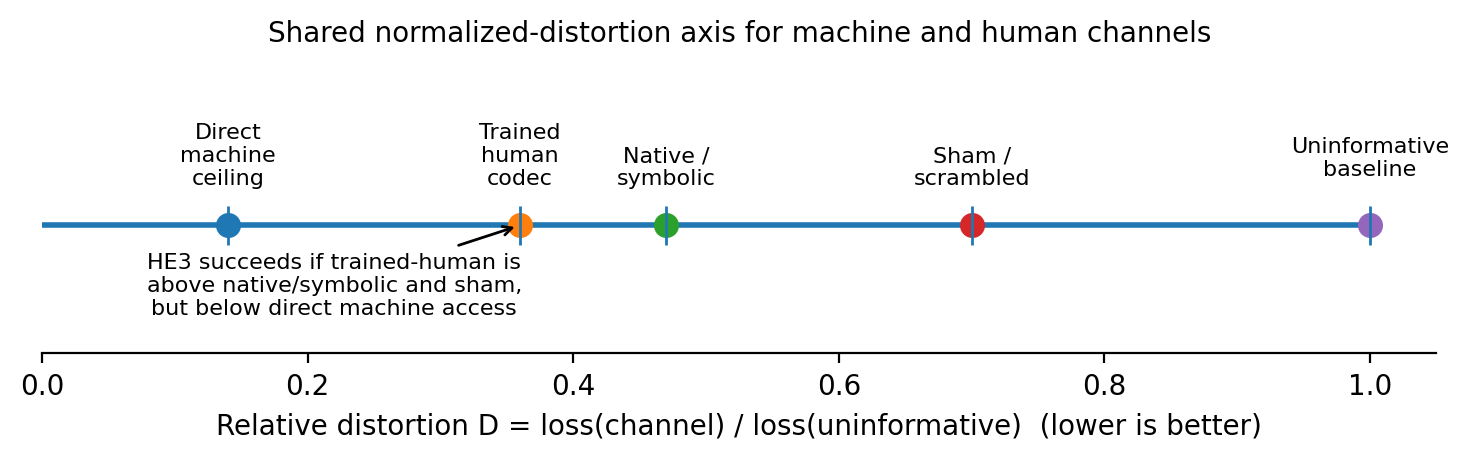
\includegraphics[keepaspectratio,alt={Figure 1. Schematic shared relative-distortion axis for HE3. Lower relative distortion is better; direct machine access defines the empirical ceiling, and the trained-human channel must land above native/symbolic and sham controls while remaining below the direct ceiling.}]{shared_normalized_distortion_axisb.png}}
\caption{Figure 1. Schematic shared relative-distortion
axis for HE3. Lower relative distortion is better;
direct machine access defines the empirical ceiling,
and the trained-human channel must land above
native/symbolic and sham controls while remaining below
the direct ceiling.}
\end{figure}

\begin{center}\rule{0.5\linewidth}{0.5pt}\end{center}

\subsection{5. Developmental feasibility: executable
proof-ladder}\label{developmental-feasibility-executable-proof-ladder}

Before human recruitment, the design was implemented as
a gated proof-ladder and run locally (numpy +
scikit-learn; Ridge for continuous targets,
distance-weighted k-NN for categorical basin/divergence
targets; eight seeds). Study 1 is run directly; Study 2
hypotheses are approximated as a machine
``human-proxy'' dry run. These numbers are
\textbf{developmental smoke-test results}, not
confirmatory evidence. The table reports the v1.3
eight-seed run after the integrity corrections of
Section 0.1; values are normalized distortion (lower is
better) unless stated.

{\def\LTcaptype{none} % do not increment counter
\begin{longtable}[]{@{}
  >{\raggedright\arraybackslash}p{(\linewidth - 6\tabcolsep) * \real{0.2500}}
  >{\raggedright\arraybackslash}p{(\linewidth - 6\tabcolsep) * \real{0.2500}}
  >{\raggedright\arraybackslash}p{(\linewidth - 6\tabcolsep) * \real{0.2500}}
  >{\raggedright\arraybackslash}p{(\linewidth - 6\tabcolsep) * \real{0.2500}}@{}}
\toprule\noalign{}
\begin{minipage}[b]{\linewidth}\raggedright
Stage
\end{minipage} &
\begin{minipage}[b]{\linewidth}\raggedright
Claim
\end{minipage} &
\begin{minipage}[b]{\linewidth}\raggedright
Developmental result (v1.3, 8 seeds)
\end{minipage} &
\begin{minipage}[b]{\linewidth}\raggedright
Gate
\end{minipage} \\
\midrule\noalign{}
\endhead
\bottomrule\noalign{}
\endlastfoot
S0 & Sanity: direct recovers; uninformative approx 1 &
direct 0.105, uninformative 1.001; per-target nRMSE
{[}spring1 0.008, spring2 0.239, coupling 0.008,
damping 0.181{]} & PASS \\
S1 & Distinction-dependence & k=2: 0.575
-\textgreater{} k=16: 0.393 & PASS \\
S2 & Throughput-invariance & delta = 0.000 (thru1x =
thru8x = 0.446) & PASS \\
S3 & Wrong-lever & hi-thru/lo-k 0.599 vs lo-thru/hi-k
0.433 & PASS \\
S4 & Corruption/divergence proxy & delta: 0.432
-\textgreater{} 0.842 -\textgreater{} 0.935 & PASS \\
S5 & Additive access proxy & native 0.533, expanded
0.529, surrogate-sham 0.534;
coupling-on-native-residual nRMSE 1.003 (no unique
signal) & \textbf{FAIL} \\
S6 & Shared placement proxy & direct 0.105 \textless{}
trained 0.423 \textless{} symbolic 0.515 & PASS \\
S7 & Dimensionality slope proxy & 4D 0.409
-\textgreater{} 8D 0.298, no degradation &
\textbf{FAIL} \\
S8 & Multi-codec audit proxy & disagreement-error corr
0.327; LOCO corr 0.615; clears permutation null (p95 =
0.073) & PASS \\
\end{longtable}
}

Two informative failures, and both are reported as
such. \textbf{S7} is the same boundary condition
documented since v1.1a: in the linear family, recovery
did not degrade as dimensionality rose; adding
oscillators supplied more informative features rather
than a harder discrimination problem. This is precisely
why the nonlinear stress-test family is required
(Appendix E), though Section 5.1 shows even the
nonlinear family does not rescue this specific gate as
written. \textbf{S5} is new to v1.3 and replaces a
previously reported PASS that depended on a weak
control. With the hardened surrogate and the
unique-contribution test, the cross-oscillator
``coupling'' channel predicts the native-channel
residual at nRMSE 1.003 - no better than the mean - so
\textbf{on the linear family} it carries no information
unique from the native channel. This is an honest
negative about that specific developmental proxy on
that source, not a confirmatory result about the human
additive-access hypothesis (HE2), which is tested
separately and under the anti-leakage discipline of
Section 6.3. The remaining gates show that the runnable
implementation is internally coherent and that the
multi-codec audit signal survives a leave-one-out and
permutation-null check; they do not show that the human
hypotheses are already supported.

\subsubsection{5.1 Cross-family generalization
(v1.4)}\label{cross-family-generalization-v1.4}

The ladder above runs on the linear calibration family.
To test whether any gate is an artifact of that single
source, v1.4 runs the full ladder across a registry of
source families and reports a gate matrix. The second
continuous family is a Duffing-type nonlinear
oscillator (cubic stiffness \texttt{-beta\ x\^{}3})
that shares the linear family's observable shape, so it
slots into the continuous-nRMSE ladder unchanged. Eight
seeds, Ridge estimator.

{\def\LTcaptype{none} % do not increment counter
\begin{longtable}[]{@{}
  >{\raggedright\arraybackslash}p{(\linewidth - 6\tabcolsep) * \real{0.2500}}
  >{\raggedright\arraybackslash}p{(\linewidth - 6\tabcolsep) * \real{0.2500}}
  >{\raggedright\arraybackslash}p{(\linewidth - 6\tabcolsep) * \real{0.2500}}
  >{\raggedright\arraybackslash}p{(\linewidth - 6\tabcolsep) * \real{0.2500}}@{}}
\toprule\noalign{}
\begin{minipage}[b]{\linewidth}\raggedright
Gate
\end{minipage} &
\begin{minipage}[b]{\linewidth}\raggedright
linear\_oscillator
\end{minipage} &
\begin{minipage}[b]{\linewidth}\raggedright
nonlinear\_oscillator
\end{minipage} &
\begin{minipage}[b]{\linewidth}\raggedright
Classification
\end{minipage} \\
\midrule\noalign{}
\endhead
\bottomrule\noalign{}
\endlastfoot
S0 sanity & PASS & PASS & family-robust \\
S1 distinction-dependence & PASS & PASS &
family-robust \\
S2 throughput-invariance & PASS & PASS &
family-robust \\
S3 wrong-lever & PASS & PASS & family-robust \\
S4 corruption-decay & PASS & PASS & family-robust \\
S5 additive-access & FAIL & PASS &
\textbf{family-specific} \\
S6 shared-placement & PASS & PASS & family-robust \\
S7 dimensionality-slope & FAIL & FAIL & fails on all \\
S8 multi-codec-audit & PASS & PASS & family-robust \\
\end{longtable}
}

Three readings, none overclaimed. (1) \textbf{Seven of
nine gates are family-robust}, so the core measurement
logic is not an artifact of the linear source. (2)
\textbf{S5 is family-specific}: cross-oscillator
coupling carries no unique signal in the linear family
but becomes informative under cubic interaction, which
supports the manuscript's premise that additive access
matters more in nonlinear regimes (HE2/HE4 motivation)
while showing the effect is family-dependent, not
universal. (3) \textbf{S7 fails on both families}: even
with nonlinearity, recovery error still falls as
oscillators are added (nonlinear trained 0.47
-\textgreater{} 0.34 across 4D-8D), because
engineered-feature count grows with oscillator count
(12 -\textgreater{} 40) faster than the nonlinearity
adds difficulty. The gate as written conflates
latent-dimension count with observable-feature count; a
corrected design (hold feature count fixed while
raising latent complexity) is listed in Future work. No
threshold was tuned per family; a FAIL is reported as a
negative.

\begin{center}\rule{0.5\linewidth}{0.5pt}\end{center}

\subsection{6. Study 2: Human codec expansion and
multi-codec
ensembles}\label{study-2-human-codec-expansion-and-multi-codec-ensembles}

\subsubsection{6.1 Objective and construct-validity
requirement}\label{objective-and-construct-validity-requirement}

Test whether participants can acquire an artificial
channel carrying a non-native distinction and whether
that acquisition improves recovery on the same held-out
source families used in Study 1. The construct-validity
requirement is \textbf{addition over substitution}: at
least one primary encoded dimension must be unavailable
to the unaided native display under the preregistered
stimulus conditions.

For the nonlinear family, non-native status is not
assumed. It is validated by a pretraining
unaided-vision baseline. A latent is eligible for HE2
only if baseline participants cannot recover it above
the preregistered threshold at the preview duration
used in the experiment. If baseline vision performs
well, that latent is demoted to a
substitution/assistive condition and is excluded from
HE2.

\subsubsection{6.2 Design}\label{design}

Three between-subjects arms:
\textbf{Expansion-trained}, \textbf{Yoked-untrained}
(equal exposure/stimulation with no informative
mapping), and \textbf{Sham-scrambled} (same
stimulation, mapping permuted each session). Practice
time is equated. Covariates include baseline working
memory, age, tactile/auditory acuity, motivation,
baseline trajectory prediction, and baseline basin
prediction. Randomization is stratified by tactile
acuity and baseline prediction; outcome assessors are
blinded to arm where feasible.

\subsubsection{6.3 Intervention}\label{intervention}

A worn 4 x 4 or 5 x 5 vibrotactile array presents a
learnable code. Substitution dimensions are retained as
secondary learnability checks. Primary addition
dimensions are basin-related and divergence-related
latents: basin label or basin probability vector;
boundary proximity or certainty; and finite-time
divergence rate. A pre-study confusion-matrix check
confirms separability of carrier frequency, rhythm,
spatial cluster, and amplitude/rhythm modulation before
the mapping is frozen. If perceptual masking is found,
the mapping is revised before confirmatory
registration.

\textbf{Anti-leakage discipline for HE2 (added v1.3).}
A developmental audit found that naively encoding the
basin label as a channel feature and then scoring
basin-label recovery is circular: the ``channel''
simply transmits the answer, and recovery is bounded
only by the encoding noise, not by any representational
acquisition. The confirmatory study therefore enforces
a separation between \emph{what the tactile channel
encodes} and \emph{what HE2b is scored on}. The channel
may carry a latent (e.g.~a basin-probability vector or
a divergence scalar), but HE2b downstream-use credit is
awarded only for predictive benefit on held-out or
near-boundary trials \textbf{whose scored target is not
the directly transmitted code} - for example,
predicting the outcome of a perturbed trajectory, or a
basin label under a stimulus regime where the encoded
probability vector is informative but not
deterministic. Direct-label transmission is treated as
an HE2a decoding check (learnability of the code),
never as evidence of representational expansion. This
mirrors the developmental \texttt{expanded\_physics}
versus \texttt{oracle\_leak\_positive\_control}
separation in Appendix F.

\subsubsection{6.4 Central
comparison}\label{central-comparison}

All channels are scored on the same held-out
trajectories. Continuous endpoints use nRMSE;
categorical basin endpoints use accuracy, Brier score,
and log-loss; all primary placements are converted to
relative distortion.

{\def\LTcaptype{none} % do not increment counter
\begin{longtable}[]{@{}
  >{\raggedright\arraybackslash}p{(\linewidth - 6\tabcolsep) * \real{0.2500}}
  >{\raggedright\arraybackslash}p{(\linewidth - 6\tabcolsep) * \real{0.2500}}
  >{\raggedright\arraybackslash}p{(\linewidth - 6\tabcolsep) * \real{0.2500}}
  >{\raggedright\arraybackslash}p{(\linewidth - 6\tabcolsep) * \real{0.2500}}@{}}
\toprule\noalign{}
\begin{minipage}[b]{\linewidth}\raggedright
Channel
\end{minipage} &
\begin{minipage}[b]{\linewidth}\raggedright
Input
\end{minipage} &
\begin{minipage}[b]{\linewidth}\raggedright
Output
\end{minipage} &
\begin{minipage}[b]{\linewidth}\raggedright
Metric
\end{minipage} \\
\midrule\noalign{}
\endhead
\bottomrule\noalign{}
\endlastfoot
Direct machine baseline & Full trajectory + simulator &
State / basin / divergence & Relative distortion;
nRMSE/log-loss panels \\
Native visual / symbolic & Short video, text, labels,
prose & State / basin guess & Relative distortion;
accuracy/log-loss \\
Trained tactile codec & Learned tactile stream carrying
eligible latents & State / basin / divergence &
Relative distortion; nRMSE/log-loss \\
Sham/scrambled tactile & Scrambled tactile stream &
State / basin guess & Relative distortion;
accuracy/log-loss \\
\end{longtable}
}

HE3 succeeds only if the trained-human channel is
measurably better than native-symbolic and sham while
remaining below the direct ceiling. The developmental
proxy placement is schematic, not a human result.

\subsubsection{6.5 Preregistered hypotheses, gated
hierarchy}\label{preregistered-hypotheses-gated-hierarchy}

Tested in order; a failed gate is reported, not
rescued.

\begin{itemize}
\tightlist
\item
  \textbf{HE1 Code learnability.} Trained participants
  decode the tactile code better than sham and transfer
  to novel exemplars, with retention at one month. This
  proves only learnability.
\item
  \textbf{HE2a Additive latent decoding.} Trained
  participants decode eligible non-native latents -
  basin-related and divergence-related quantities that
  failed the native-vision baseline - better than
  native-only and sham.
\item
  \textbf{HE2b Downstream use.} The trained channel
  improves prediction or reconstruction on held-out or
  near-boundary trials beyond what is explained by
  decoding visible parameters alone. This is the
  stronger codec-expansion test.
\item
  \textbf{HE3 Shared rate-distortion placement.} The
  trained-human channel occupies an intermediate
  position on the Study 1 relative-distortion curve:
  worse than direct machine access, better than
  native/symbolic and sham.
\item
  \textbf{HE4 Dimensionality and complexity scaling.}
  As calibrated dynamical complexity rises, trained
  recovery degrades but remains above control over at
  least part of the range. The primary slope is
  analyzed against measured complexity, with magnet
  count as a planned secondary index.
\item
  \textbf{HE5 Multi-codec audit value.} Independent
  projections reduce undetected high-error cases
  relative to any single human-readable projection.
  Primary statistics: disagreement-error correlation,
  AUC for detecting top-quartile true error, and
  reduction in high-confidence/high-error cases. Ranked
  last because it is model-dependent.
\end{itemize}

For HE3/HE4 the central-rate plateau is estimated from
data, not fixed to a literature constant.

\subsubsection{6.6 Predicted dimensionality pattern in
the nonlinear stress
test}\label{predicted-dimensionality-pattern-in-the-nonlinear-stress-test}

{\def\LTcaptype{none} % do not increment counter
\begin{longtable}[]{@{}
  >{\raggedright\arraybackslash}p{(\linewidth - 8\tabcolsep) * \real{0.2000}}
  >{\raggedright\arraybackslash}p{(\linewidth - 8\tabcolsep) * \real{0.2000}}
  >{\raggedright\arraybackslash}p{(\linewidth - 8\tabcolsep) * \real{0.2000}}
  >{\raggedright\arraybackslash}p{(\linewidth - 8\tabcolsep) * \real{0.2000}}
  >{\raggedright\arraybackslash}p{(\linewidth - 8\tabcolsep) * \real{0.2000}}@{}}
\toprule\noalign{}
\begin{minipage}[b]{\linewidth}\raggedright
Complexity stratum
\end{minipage} &
\begin{minipage}[b]{\linewidth}\raggedright
Native visual
\end{minipage} &
\begin{minipage}[b]{\linewidth}\raggedright
Sham tactile
\end{minipage} &
\begin{minipage}[b]{\linewidth}\raggedright
Trained tactile
\end{minipage} &
\begin{minipage}[b]{\linewidth}\raggedright
Machine baseline
\end{minipage} \\
\midrule\noalign{}
\endhead
\bottomrule\noalign{}
\endlastfoot
Low calibrated complexity & Moderate & No gain &
Significant gain & Best \\
Medium calibrated complexity & Weaker & No gain &
Partial gain & Best \\
High calibrated complexity & Weak & No gain & Degraded
but above control if expansion scales & Best \\
\end{longtable}
}

The slope matters more than any single point. A clean
low-complexity success with high-complexity collapse
supports learnability but weakens the
superintelligence-relevant extrapolation; the program
reports it as such.

\subsubsection{6.7 Measures, controls, power,
ethics}\label{measures-controls-power-ethics}

Measures are kept distinct: repertoire (unspeeded
absolute identification, bits transferred), central
rate (bits/s under speeded feedback-withheld
conditions), recovery (relative distortion through the
trained channel), and communication payoff
(relay/ensemble performance). Sham isolates distinction
acquisition from arousal and novelty; yoked isolates
exposure; total minutes are equated; within-session
sham learnability is analyzed rather than assumed away.

The target is \textbf{90-105 completers} (30-35 per
arm). With 25-30\% attrition expected for a demanding
10-12 session protocol, enrollment should be planned at
approximately 120-150 participants unless replacement
is continuous. Primary HE1/HE2 contrasts are powered
for \texttt{d\ approx\ 0.5}; HE3/HE4/HE5 use frozen
simulation-based curves. Bayesian Bayes factors are
reported alongside frequentist tests.

Hardware is consumer-grade, non-invasive,
amplitude-limited, with participant stop, thermal
monitoring, and skin checks. The protocol is intended
for low-risk human-subjects review. Failure of
motivated participants to learn the mapping is itself a
meaningful boundary condition.

\begin{center}\rule{0.5\linewidth}{0.5pt}\end{center}

\subsection{7. Analysis plan and inferential
discipline}\label{analysis-plan-and-inferential-discipline}

Study 1 uses paired comparisons across held-out
trajectories, bootstrap confidence intervals,
mixed-effects models, and TOST for
throughput-invariance. The main estimand is the
relative contribution of \texttt{k} and \texttt{C\_io}
to relative distortion after intake saturation. For the
magnetic-pendulum family, complexity calibration is
completed before confirmatory testing and then frozen.

Study 2 uses mixed-effects models with participant
random effects; fixed effects for arm, complexity,
session, channel, and preregistered covariates. Basin
targets use logistic or multinomial mixed models plus
log-loss/Brier analyses. Continuous targets use nRMSE
and relative distortion. HE3 places each human channel
on the Study 1 axis with confidence intervals. HE4
estimates the slope across calibrated complexity. HE5
compares single- vs multi-codec ensembles on undetected
high-error cases, disagreement-error correlation, and
top-error AUC.

Multiplicity is controlled by the gated hierarchy: if
HE1 fails, HE2-HE5 are exploratory; if HE2 fails, HE3
cannot be read as codec expansion; if the
native-invisibility check fails for a latent, that
latent cannot support HE2.

\begin{center}\rule{0.5\linewidth}{0.5pt}\end{center}

\subsection{8. Safety implication: codec contrast as a
measurable audit
layer}\label{safety-implication-codec-contrast-as-a-measurable-audit-layer}

A single human-readable channel can create false
transparency: the system seems interpretable because it
is fluent, while operative structure remains outside
the receiving codec. Multi-codec contrast mitigates
this by requiring independent projections - symbolic,
visual/geometric, mathematical, causal-graph,
simulated, and eventually trained-sensory - whose
agreements and disagreements are inspected.

\textbf{Codec-contest principle.} If a system's
internal structure cannot be directly inspected,
require multiple independent human-auditable
projections and test whether they remain mutually
consistent under perturbation. Inconsistency is
evidence of translation loss, underspecification,
projection-dependent omission, or possible strategic
misdirection; it is not, by itself, proof of deception,
and it is not a solution to alignment, corrigibility,
or governance.

HE5 makes one audit layer measurable. The developmental
proxy run showed a positive disagreement-error
correlation (0.75 against the ensemble's own error)
that survives two falsification checks added in v1.3: a
leave-one-codec-out estimate (0.62), in which a
held-out codec's error is predicted from the
disagreement of the \emph{other} codecs only, and a
permutation null whose 95th percentile (0.07) the
observed correlation clears on every seed. These checks
rule out the concern that the correlation is a
mechanical artifact of comparing a cross-codec standard
deviation with a deviation of the same codecs' mean
from truth. They do not make the result confirmatory.
They also do not retire the central caveat:
developmental mean pairwise codec-error correlation was
0.57, so the codecs share substantial error, and
\emph{agreement} among correlated codecs can be
confidently wrong. The audit's value lies in
disagreement predicting error, not in agreement
certifying correctness. The confirmatory question
remains whether disagreement flags otherwise undetected
high-error cases under preregistered conditions, with
correlated error reported as the primary failure mode.

\begin{center}\rule{0.5\linewidth}{0.5pt}\end{center}

\subsection{9. Discussion}\label{discussion}

\textbf{The empirical spine.} The program now rests on
five linked choices: (1) Study 1 and Study 2 share
source families and metrics; (2) Study 2 promotes at
least one dimension from substitution to validated
addition; (3) the linear family is used for calibration
while the nonlinear family supplies the stress test for
HE2/HE4; (4) a runnable proof-ladder validates
implementation before human data; and (5) hypotheses
are gated so downstream claims cannot rescue upstream
failures.

\textbf{Repertoire vs throughput.} Study 2 clarifies
rather than contradicts the throughput critique. The
binding variable is \texttt{k}, the repertoire of
usable distinctions. New distinctions may arrive via
tactile language, AR interface, auditory code,
mathematical tool, team protocol, or cortical implant -
different delivery routes to the same variable,
compared on acquisition speed, dimensionality,
retention, risk, and burden.

\textbf{Reach frontiers vs horizons, with chaos.} Both
studies probe reach frontiers, not horizons. Expansion
raises \texttt{rho} toward a higher ceiling, not to 1.
The chaotic medium is constrained by the Lyapunov-time
discipline so it never silently becomes a horizon-like
regime that floors all codecs.

\textbf{What would falsify the program.} HE1 failure
means the tactile code is not learnable in this regime.
HE2 failure means the added channel does not expand
recoverable distinctions beyond practice or arousal.
HE3 failure collapses the shared-axis claim. HE4
flat-good or flat-bad results weaken the scaling
inference. S1-H2 failure would revive throughput as a
live competing explanation.

\textbf{Limitations.} Tactile dimensionality is low;
acquisition is slow and variable; the central rate may
hard-cap real-time depth regardless of repertoire;
\texttt{rho}, distinction count, and relative
distortion are operational proxies; HE5 uses model
projections, not a superintelligence; chaotic targets
must remain inside the Lyapunov window; feasibility at
scale is partly untested; and physical pendulum
demonstrations cannot provide confirmatory ground
truth.

\textbf{Future work.} Natural-language baselines under
matched budgets; additional chaotic and PDE families
folded into the cross-family registry (extending the
v1.4 two-family pass, Section 5.1); an S7 redesign that
holds observable-feature count fixed while raising
latent complexity, so the dimensionality slope is
measurable rather than confounded by feature growth
(per the v1.4 finding); real sensor streams; a
dedicated dimensionality-scaling study with stronger
encoders; a trans-codec agent benchmark; and
head-to-head comparison of non-invasive and invasive
delivery routes once both are mature.

\begin{center}\rule{0.5\linewidth}{0.5pt}\end{center}

\subsection{10. Conclusion}\label{conclusion}

Superintelligence may be marked not only by superior
problem-solving but by machine-native distinctions that
cannot be faithfully compressed into unaided human
channels. When such distinctions exceed the human
codec, explanation becomes a lossy projection and the
danger is false transparency.

The proposed experiments test the minimal bridge: Study
1 builds a machine rate-distortion frontier for
held-out dynamical systems; Study 2 asks whether a
trained human, via an artificial tactile channel
carrying a validated non-native latent, can move along
that same frontier. Success would not prove that humans
can understand arbitrary superintelligence. It would
prove something narrower but important: human
representational reach is experimentally expandable and
measurable.

The safety implication is that oversight should not
rely on a single explanation channel. It should require
multi-codec projections whose consistency and
disagreement signals can be audited. The broader
implication remains conditional: preserving human
agency under future machine-native cognition may
require expanding the human codec, but the present
studies only test the first measurable step.

\begin{center}\rule{0.5\linewidth}{0.5pt}\end{center}

\subsection{Appendix A. Tactile language training
protocol}\label{appendix-a.-tactile-language-training-protocol}

\textbf{A.1 Hardware.} Voice-coil tactors in a 4 x 4 or
5 x 5 array, approximately 2.5 cm spacing, worn on the
volar forearm or abdomen; driver \textgreater= 200 Hz
update, \textgreater= 8-bit amplitude, independent
channels; amplitude within safety range; thermal
monitoring; participant stop.

\textbf{A.2 Encoding baseline.} Substitution dimensions
are secondary: spring or visible parameter
-\textgreater{} carrier frequency; damping
-\textgreater{} duty cycle; coupling -\textgreater{}
spatial location; drive or source family marker
-\textgreater{} amplitude modulation. Addition
dimensions are primary only after native-invisibility
validation: basin label or basin probability vector
-\textgreater{} reserved burst rhythm or tactor
cluster; boundary proximity/certainty -\textgreater{}
rhythm density; finite-time divergence -\textgreater{}
amplitude/rhythm modulation. Perceptual independence is
confirmed by a pre-study confusion matrix.

\textbf{A.3 Curriculum.} Ten to twelve sessions: S1-S3
single-feature identification; S4-S6 two-feature
conjunctions and mid-training retention probe; S7-S8
latent-variable introduction; S9-S10 full trajectories
with fading visual support; S11-S12 novel exemplars,
retention, and ensemble-channel introduction. Feedback
is immediate early and faded later. Home practice, if
used, is monitored and analyzed separately.

\textbf{A.4 Controls.} Sham-scrambled: same
hardware/time/interface, mapping permuted each session.
Yoked-untrained: same stimulation/time, non-informative
source, framed neutrally.

\begin{center}\rule{0.5\linewidth}{0.5pt}\end{center}

\subsection{Appendix B. Power and sample
size}\label{appendix-b.-power-and-sample-size}

The primary HE1/HE2 contrast is trained vs control,
powered for \texttt{d\ approx\ 0.5-0.6}, 80\% power,
two-sided alpha = 0.05. The target is 30-35 completers
per arm, 90-105 completers total. With 25-30\%
attrition, planned enrollment should be approximately
120-150 unless replacement enrollment is continuous.
HE3 placement, HE4 slope, and HE5 audit are powered via
frozen simulation curves. Rate-plateau equivalence uses
a preregistered TOST margin with sensitivity analyses;
Bayesian Bayes factors are reported.

\begin{center}\rule{0.5\linewidth}{0.5pt}\end{center}

\subsection{Appendix C. Response-to-reviewer
record}\label{appendix-c.-response-to-reviewer-record}

We accept exposition and design clarifications:
corrected cosmology mapping, safety-audit framing,
shared-axis unification, addition-over-substitution,
dimensionality slope, confusion-matrix pre-check, gated
hierarchy, nonlinear stress-test source family,
executable proof-ladder, native-invisibility
validation, calibrated complexity, and normalized
relative distortion.

We do \textbf{not} adopt claims that biological
integration is necessary for survival, that any
specific BCI program is privileged, or that codec
contrast is a complete safety solution. These exceed
the evidential scope. The central claim remains:
human-compatible reach frontiers can be experimentally
measured, and artificial channels may expand the
distinctions humans recover under controlled
conditions.

{\def\LTcaptype{none} % do not increment counter
\begin{longtable}[]{@{}
  >{\raggedright\arraybackslash}p{(\linewidth - 2\tabcolsep) * \real{0.5000}}
  >{\raggedright\arraybackslash}p{(\linewidth - 2\tabcolsep) * \real{0.5000}}@{}}
\toprule\noalign{}
\begin{minipage}[b]{\linewidth}\raggedright
Recommendation
\end{minipage} &
\begin{minipage}[b]{\linewidth}\raggedright
Decision
\end{minipage} \\
\midrule\noalign{}
\endhead
\bottomrule\noalign{}
\endlastfoot
Unify on shared trajectories/metric & Accepted \\
Substitution -\textgreater{} addition & Accepted, with
native-invisibility validation \\
Dimensionality slope & Accepted, with calibrated
complexity \\
Confusion-matrix pre-check & Accepted \\
Gated hierarchy & Accepted \\
Corrected cosmology mapping & Accepted \\
Codec contrast as audit layer & Accepted, portfolio
framing \\
Nonlinear magnetic-pendulum source & Accepted as stress
test, not broad proxy for SI \\
Executable proof-ladder & Accepted as developmental
smoke test \\
Developmental additive-access leakage (self-audit,
v1.3) & Accepted; channel rebuilt without target, leak
retained as labeled control (Appendix F) \\
Multi-codec audit possibly tautological (self-audit,
v1.3) & Accepted; LOCO + permutation null added, signal
survives (Appendix F) \\
Single-source-family limitation (self-audit, v1.4) &
Accepted; cross-family registry + gate matrix added,
7/9 gates family-robust (Section 5.1, Appendix F.6) \\
Survival necessity & Rejected \\
Bach-y-Rita as survival prototype & Reframed \\
Codec contrast as only deception detector & Softened \\
All resources to one device program / fixed 39-bit
constant & Rejected / reframed \\
\end{longtable}
}

\begin{center}\rule{0.5\linewidth}{0.5pt}\end{center}

\subsection{Appendix D. Preregistration
checklist}\label{appendix-d.-preregistration-checklist}

Freeze simulator code, seeds, and solver tolerances
before confirmatory Study 1. Freeze the held-out source
families and reuse them identically in Study 2. Freeze
the native-invisibility thresholds and baseline preview
duration. Freeze the tactile mapping after
perceptual-independence testing. Define native-only,
symbolic, sham, trained, and direct channels before
collection. Register S1-H1-H4 and HE1-HE5 primary
outcomes. Register the Lyapunov-time window, basin
metrics, and complexity index. Register equivalence
margins and effect-size floors. Register attrition
replacement and unusable-session stopping rules.
Register exclusions for device intolerance, incomplete
sessions, failed attention checks, and technical
failures. Deposit analysis, figure, power, and
proof-ladder code on OSF. Preserve Appendix C as
claim-hygiene documentation.

\begin{center}\rule{0.5\linewidth}{0.5pt}\end{center}

\subsection{Appendix E. Developmental proof-ladder
notes}\label{appendix-e.-developmental-proof-ladder-notes}

The proof-ladder is useful because it gives the program
a falsifiable implementation skeleton before human
collection. It should not be described as proof of the
human hypotheses. The following corrections are
required for the confirmatory version. Items 4-5 were
applied to the developmental code in v1.3; items 1-3
remain confirmatory-only requirements.

\begin{enumerate}
\def\labelenumi{\arabic{enumi}.}
\tightlist
\item
  S2 equivalence must use a full TOST confidence
  interval, not only a point-delta check.
\item
  S4 must use actual measurement-basis rotations for
  divergence; the developmental corruption step is only
  a proxy.
\item
  S7 must run on the calibrated nonlinear source
  family, because the linear source family did not
  generate the required difficulty slope.
\item
  (Applied v1.3) Any ``additive-access'' or
  ``expanded'' channel must be built from observables
  that exclude the scored target. The developmental
  code now separates an \texttt{expanded\_physics}
  channel from an explicitly labeled
  \texttt{oracle\_leak\_positive\_control}; the
  confirmatory tactile mapping inherits the
  anti-leakage discipline of Section 6.3.
\item
  (Applied v1.3) Additive-access controls must be
  distribution-preserving (phase-randomized surrogate)
  rather than a destructive reshuffle, and must include
  a unique-contribution test against the native-channel
  residual. The developmental S5 now reports an honest
  negative under these controls.
\end{enumerate}

\begin{center}\rule{0.5\linewidth}{0.5pt}\end{center}

\subsection{Appendix F. Developmental integrity audit
(v1.3)}\label{appendix-f.-developmental-integrity-audit-v1.3}

Before submission, the developmental code was subjected
to an adversarial self-audit aimed at finding leakage,
circular controls, and overclaimed proxies. The audit
changed developmental numbers but no confirmatory
claim. It is recorded here for claim hygiene; full
diagnostics and before/after artifacts are deposited
with the analysis code.

\textbf{F.1 Critical finding - target leakage in the
developmental magnetic ``expanded'' channel.} The
pre-v1.3 channel concatenated a noisy one-hot copy of
the basin label and a noisy copy of the finite-time
divergence target into its own feature matrix. A
classifier given \emph{only} that leaked channel, with
no physics features, reached basin accuracy 0.87 at
five magnets against a noise ceiling of
\texttt{1\ -\ flip\_prob\ =\ 0.88}. The earlier
``expanded beats native'' reading was therefore an
artifact of transmitting the answer, not evidence of
representational access. Mitigation: the leaked channel
is retained only as
\texttt{oracle\_leak\_positive\_control} (a ceiling
check), and an honest \texttt{expanded\_physics}
channel was built from additional preview observables
(velocity-profile statistics, speed extrema,
radial-distance dynamics, a cross-coordinate
interaction moment) containing no target. Under the
honest channel, expanded physics does not beat the
native preview (mean basin-accuracy delta -0.029 across
\texttt{m\ =\ 3,\ 4,\ 5}); the full-trajectory
\texttt{direct} channel is best. The corrected
developmental gate now passes on an honest criterion
(stays above chance + 0.20 and degrades gracefully,
drop 0.07 across the range, no collapse), and the
confirmatory human protocol inherits the anti-leakage
rule in Section 6.3.

\textbf{F.2 Additive-access control (S5).} The prior
sham used an independent train/test reshuffle, which
reduces to ``native plus noise'' rather than ``native
plus a distribution-matched but target-misaligned
channel.'' Mitigation: a phase-randomized surrogate
that preserves each feature's marginal distribution,
plus a unique-contribution test (predict the
native-channel residual from the candidate channel). On
the linear family the coupling channel predicts the
residual at nRMSE 1.003 - no better than the mean - so
S5 is now an honest FAIL: the coupling channel carries
no information unique from the native channel in this
medium.

\textbf{F.3 Multi-codec audit (S8 / HE5 proxy).} The
developmental disagreement-error correlation is
measured against the ensemble's own error, which raises
a tautology concern. Two checks were added. A
leave-one-codec-out estimate predicts each held-out
codec's error from the disagreement of the other codecs
only (0.62); a permutation null gives a 95th-percentile
correlation of 0.07, which the observed value clears on
every seed. A synthetic control confirmed that pure
common-mode error does \textbf{not} induce the
correlation. The signal is therefore genuine
heteroscedasticity, not an artifact - while the
correlated-error caveat (mean pairwise codec-error
correlation 0.57) remains the primary failure mode.

\textbf{F.4 Reporting discipline.} Developmental seeds
were raised from two to eight; per-target normalized
distortion is now reported for S0 (revealing, for
example, that damping and one spring constant are
materially harder to recover than the others, which a
scalar mean had hidden); and across-seed standard
deviations accompany the headline developmental
metrics.

\textbf{F.5 Open item (closed in v1.4).} The single
largest remaining limitation of the v1.3 developmental
skeleton was that every stage drew from one source
family at a time. v1.4 closes this: the ladder runs
across a source-family registry behind one switch, with
a regression fixture freezing the linear numbers and a
per-family no-leakage test preventing reintroduction of
F.1. See F.6 and Section 5.1.

\textbf{F.6 Cross-family generalization (v1.4).} A
\texttt{SourceFamily} protocol now routes data
production; the linear family delegates to the original
code (verified byte-identical against a frozen
fixture), and a Duffing-type nonlinear oscillator was
added. Running both families through the ladder shows
seven of nine gates family-robust (S0-S4, S6, S8). Two
honest results emerged that the single-family setup
could not surface: S5 (additive-access) is
family-specific - it FAILs on the linear family but
PASSes on the nonlinear one, where cubic coupling is
informative - and S7 (dimensionality slope) FAILs on
both families because engineered-feature count grows
with oscillator count faster than the nonlinearity adds
difficulty (a gate-design conflation now flagged for
redesign). The implementation, gate matrix, and seven
new tests are deposited with the analysis code; no gate
threshold was tuned per family.

\begin{center}\rule{0.5\linewidth}{0.5pt}\end{center}

\subsection{References}\label{references}

Bach-y-Rita, P., Collins, C. C., Saunders, F. A.,
White, B., \& Scadden, L. (1969). Vision substitution
by tactile image projection. \emph{Nature, 221}(5184),
963-964.

Bostrom, N. (2014). \emph{Superintelligence: Paths,
Dangers, Strategies}. Oxford University Press.

Coupé, C., Oh, Y. M., Dediu, D., \& Pellegrino, F.
(2019). Different languages, similar encoding
efficiency: Comparable information rates across the
human communicative niche. \emph{Science Advances,
5}(9), eaaw2594.

Cover, T. M., \& Thomas, J. A. (2006). \emph{Elements
of Information Theory} (2nd ed.). Wiley.

Eagleman, D. M., \& Perrotta, M. V. (2023). The future
of sensory substitution, addition, and expansion via
haptic devices. \emph{Frontiers in Human Neuroscience,
16}.

Lachmann, M., Newman, M. E. J., \& Moore, C. (2004).
The physical limits of communication. \emph{American
Journal of Physics, 72}(10), 1290-1293.

Satz, W. A. (2026). \emph{The Codec Ceiling: A
Preregistered Description-Channel Gap in Coupled
Oscillators}. Preprint.

Shannon, C. E. (1948). A mathematical theory of
communication. \emph{Bell System Technical Journal,
27}(3), 379-423; \emph{27}(4), 623-656.

Strogatz, S. H. (2015). \emph{Nonlinear Dynamics and
Chaos} (2nd ed.). Westview Press.

Zheng, J., \& Meister, M. (2025). The unbearable
slowness of being: Why do we live at 10 bits/s?
\emph{Neuron, 113}(2), 192-204.

\end{document}
